\documentclass{beamer}

\usepackage[english,russian]{babel}
\usepackage[utf8]{inputenc}

\usepackage{amsmath}
\numberwithin{equation}{section}

\usepackage{graphicx}
\usepackage{epstopdf} 

\usetheme{Warsaw}
\usecolortheme{beaver}
\useoutertheme{miniframes}
\setbeamertemplate{navigation symbols}{}

\setbeamertemplate{headline}
{%\
    \begin{beamercolorbox}[ht=2.25ex,dp=1.1ex]{section in head/foot}
        \insertsectionnavigationhorizontal{\paperwidth}{}{\hfill\hfill}
    \end{beamercolorbox}%
}

\setbeamertemplate{footline}
{%\
    \begin{beamercolorbox}{section in head/foot}
        \text{ } \insertshorttitle \hfill \insertframenumber \text{ }
    \end{beamercolorbox}%
}

\begin{document}
    
    \title{Особенности математических моделей теплопроводности с отклоняющимся аргументом}
    
    \author{Качалкин Иван}
    
    \institute{Московский государственный университет путей сообщения (МИИТ)\\Кафедра ``Прикладная математика-1''\\
        \vspace{0.7cm}
        Научный руковдитель: профессор, д.ф.-м.н. Филимонов А.М.
        \vspace{0.7cm}
    }
    
    \date{июнь 2014}

    {
        \setbeamertemplate{footline}{} 
        \setbeamertemplate{headline}{}
        \frame{\titlepage}
    }

    \section{Постановка задачи}
    \subsection{Математическая модель задачи}
    \begin{frame}
        \frametitle{Постановка задачи}
        \framesubtitle{Исходные уравнения}

        \textbf{Общее уравнение непрерывности} в дифференциальной форме:

        \begin{equation}
            \rho_t + div \bar{J} = f \text{,}
        \end{equation}

        где \textbf{плотность потока} $\bar{J}$ выражена законом диффузии с конвекцией ($\rho$ \--- температура):

        \begin{equation}
            \bar{J}(x,t) = -a^2 \nabla \rho(x,t) + \bar{V}(x,t) \rho(x,t)
        \end{equation}

    \end{frame}

    \subsection{Уравненение диффузии с запаздыванием}
    \begin{frame}
        \frametitle{Постановка задачи}
        \framesubtitle{Уравненение диффузии с запаздыванием}

        Рассмотрим закон теплопроводности с отклонением по времени:

        \begin{equation}
            \bar{J}(x,t+\tau) = -a^2 \nabla \rho(x,t) + \bar{V}(x,t) \rho(x,t)
        \end{equation}

        \begin{equation}
            \sum\limits_{n=0}^{m} \dfrac{\partial^n \bar{J}}{\partial t^k}(x,t) \dfrac{\tau^n}{n!} = -a^2 \nabla \rho(x,t) + \bar{V}(x,t) \rho(x,t)
        \end{equation}

        \begin{equation}
            \sum\limits_{n=0}^{m} \dfrac{\partial^{n+1} u}{\partial t^{n+1}} \dfrac{\tau^n}{n!} - a^2 \dfrac{\partial^2 u}{\partial x^2} + \dfrac{V^2}{4a^2} u = 0
        \end{equation}

        \begin{equation}
            \rho(x,t) = e^{\xi x} u(x,t)
        \end{equation}

    \end{frame}

    \section{Приближения ОДУ}
    \subsection{Сведение к исследованию ОДУ методом Фурье и исследование его усточивости по критерию Рауса-Гурвица}
    \begin{frame}
        \frametitle{Исследование устойчивости приближений}
        \framesubtitle{Сведение к исследованию ОДУ методом Фурье и исследование его усточивости по критерию Рауса-Гурвица}

        \begin{equation}
            \left\{
            \begin{aligned}
                \sum\limits_{k=0}^{m} \dfrac{\tau^k}{k!} T^{(k+1)} + \underbrace{ \left( \dfrac{V^2}{4a^2} + a^2 k^2 \right)}_{\gamma(k)} T & = 0\\
                X'' + k^2 X & = 0
            \end{aligned}
            \right.
        \end{equation}

        \begin{equation}
            \sum\limits_{k=0}^{m} \dfrac{\tau^k}{k!} \lambda^{k+1} + {\gamma} = 0
        \end{equation}

    \end{frame}

    \subsection{Критерий Рауса-Гурвица}

    \begin{frame}
        \frametitle{Исследование устойчивости приближений}
        \framesubtitle{Критерий Рауса-Гурвица}

        \begin{equation}
            a_0 y^n + a_1 y^{n-1} + \dots + a_{n-1} y + a_n = 0 \quad a \neq 0
        \end{equation}
    
        \begin{align*}
            & \Delta_0 = a_0 > 0, \quad \Delta_1 = a_1, \quad \Delta_2 = 
            \begin{vmatrix}
                a_1 & a_0\\
                a_3 & a_2
            \end{vmatrix},\\
            & \Delta_3 = 
            \begin{vmatrix}
                a_1 & a_0 & 0\\
                a_3 & a_2 &a_1\\
                a_5 & a_4 &a_3
            \end{vmatrix}, \quad \Delta_4 =
            \begin{vmatrix}
                a_1 & a_0 & 0 & 0\\
                a_3 & a_2 & a_1 & a_0\\
                a_5 & a_4 & a_3 & a_2\\
                a_7 & a_6 & a_5 & a_4
            \end{vmatrix}, \dots
        \end{align*}
    \end{frame}

    \subsection{Результаты численного исследования}
    \begin{frame}
        \frametitle{Исследование устойчивости приближений}
        \framesubtitle{Результаты численного исследования}

        \begin{small}

        \textbf{при $m=1$}: $\Delta_1 = 1 > 0$, $\Delta_1 = \gamma > 0$\\

        \textbf{при $m=2$}: $\Delta_1 = \tau$, $\Delta_2 = \tau (1 - 0.5 \gamma \tau) < 0$, $\Delta_3 = \gamma \tau (1 - 0.5 \gamma \tau) < 0$\\

        \textbf{при $m=3$}: $\Delta_1 = 0.5 \tau ^2$, $\Delta_2 \approx 0.33 \tau ^3$, $\Delta_3 \approx \tau ^3 (0.33\, -0.25 \gamma  \tau ) < 0$, $\Delta_4 \approx \gamma  \tau ^3 (0.33\, -0.25 \gamma  \tau ) < 0$\\

        \textbf{при $m=4$}: $\Delta_1 = 0.167 \tau ^3$, $\Delta_2 = 0.041 \tau ^5$, $\Delta_3 = \tau ^6 (0.007 \gamma  \tau + 0.014)$, \\$\Delta_4 = \tau ^6 \left(-0.0017 \gamma ^2 \tau ^2-0.007 \gamma  \tau +0.014\right) < 0$, $\Delta_5 = \gamma  \tau ^6 \left(-0.0017 \gamma ^2 \tau ^2-0.0071 \gamma  \tau +0.0139 \right)$\\

        \textbf{при $m=5$}: $\Delta_1 = 0.042 \tau ^4$, $\Delta_2 = 0.003 \tau ^7$, $\Delta_3 = 0$, $\Delta_4 = \tau ^{10} (0.0001 \gamma  \tau -0.0002)$, $\Delta_5 = \tau ^{10} \left(-0.0001 \gamma ^2 \tau ^2+0.0002 \gamma  \tau -0.0002\right) < 0$, \dots\\

        \textbf{при $m=6$}: $\Delta_1 = 0.0083 \tau ^5$, $\Delta_2 = 0.0001 \tau ^9$, $\Delta_3 = -3.858^{-6} \tau ^{12} < 0$, \dots\\

        \textbf{при $m=7$}: $\Delta_1 = 0.00138889 \tau ^6$, $\Delta_2 = 3.307^{-6} \tau ^{11}$, $\Delta_3 = -4.593^{-8} \tau ^{15} < 0$, \dots\\

        \end{small}

    \end{frame}

    \subsection{Аналитическое доказательство неустойчивости приближений}
    \begin{frame}
        \frametitle{Исследование устойчивости приближений}
        \framesubtitle{Аналитическое доказательство неустойчивости приближений}

        \textbf{Утверждение}. $\Delta_3 < 0$ при $m \geq 6$.

        \begin{equation}
            \Delta_3 = 
            \begin{vmatrix}
                \frac{\tau^{m-1}}{(m-1)!} & \frac{\tau^{m}}{m!} & 0\\
                \frac{\tau^{m-3}}{(m-3)!} & \frac{\tau^{m-2}}{(m-2)!} & \frac{\tau^{m-1}}{(m-1)!}\\
                \frac{\tau^{m-5}}{(m-5)!} & \frac{\tau^{m-4}}{(m-4)!} & \frac{\tau^{m-3}}{(m-3)!}
            \end{vmatrix} =
            \dfrac{\tau^{3m-6}}{m!(m-1)!(m-3)!} (10-2m) < 0
        \end{equation}

        \begin{center}
            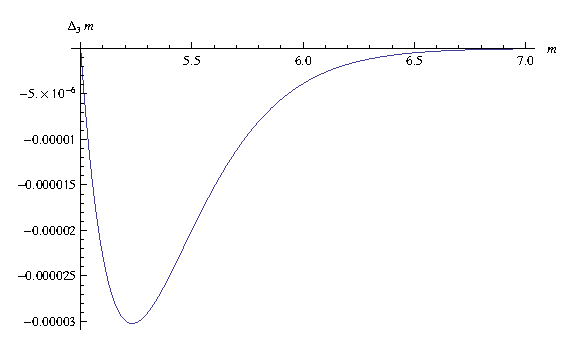
\includegraphics[width=0.65\textwidth]{coefCheck.eps}
        \end{center}
    
    \end{frame}

    \section{Уравнение с запаздыванием}

    \subsection{Переход к исследованию системы ОДУ с запаздыванием}

    \begin{frame}
        \frametitle{Исследование уравнения с запаздыванием}
        \framesubtitle{Переход к исследованию системы ОДУ с запаздыванием}

        \begin{equation}
            u_t (x,t) - a^2 u_{xx} (x,t-\tau) + \dfrac{V^2}{4a^2} u (x,t-\tau) = 0
        \end{equation}

        \begin{equation}
            \left\{
            \begin{aligned}
                T'(t) + \underbrace{ \left( \dfrac{V^2}{4a^2} + a^2 k^2 \right)}_{\gamma(k^2)} T(t-\tau) & = 0\\
                X'' + k^2 X & = 0
            \end{aligned}
            \right.
        \end{equation}
    \end{frame}

    \subsection{Задача Коши для уравнения с запаздыванием}

    \begin{frame}
        \frametitle{Уравнение с запаздыванием}
        \framesubtitle{Задача Коши для уравнения с запаздыванием}

        \begin{equation}
            \left\{
            \begin{aligned}
                T'_k (t) + \underbrace{ \left( \dfrac{V^2}{4a^2} + a^2 k^2 \right)}_{\gamma(k^2)} T_k (t-\tau) = 0, \quad t>0,\\
                T_k (t) = T_{k}^{0}, \quad -\tau \leq t \leq 0.
            \end{aligned}
            \right.
        \end{equation}

        На основании \textbf{теоремы Руше} получено достаточное условие устойчивости решений:

        \begin{equation}
            \gamma(k^2) \tau < 1
        \end{equation}
    \end{frame}

    \subsection{Cравнение с различными приближениями}

    \begin{frame}
        \frametitle{Исследование уравнения с запаздыванием}
        \framesubtitle{Сравнение с различными приближениями}

        \begin{figure}[h]
        \begin{center}
            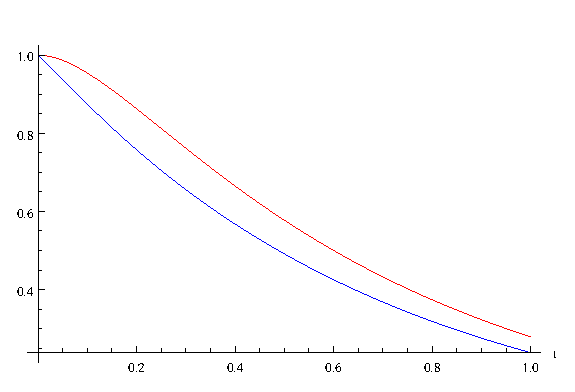
\includegraphics[width=0.65\textwidth]{example_trivia.eps}
        \end{center}
        \caption{При $\tau=0.1$, $k=1$, $m=1$}
        \end{figure}
    \end{frame}

    \begin{frame}
        \frametitle{Исследование уравнения с запаздыванием}
        \framesubtitle{Сравнение с различными приближениями}

        \begin{figure}[h]
        \begin{center}
            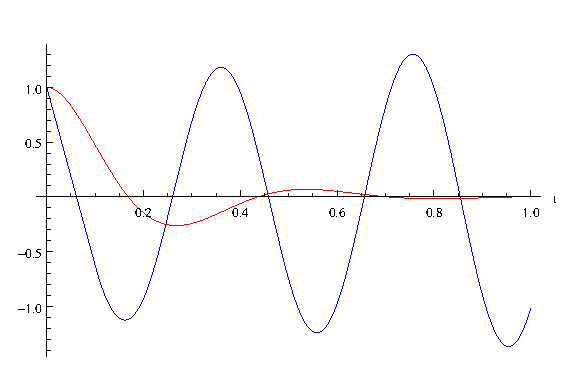
\includegraphics[width=0.65\textwidth]{example_trivia_bad.eps}
        \end{center}
        \caption{При $\tau=0.1$, $k=4$, $m=1$}
        \end{figure}
    \end{frame}

    \begin{frame}
        \frametitle{Исследование уравнения с запаздыванием}
        \framesubtitle{Сравнение с различными приближениями}

        \begin{figure}[h]
        \begin{center}
            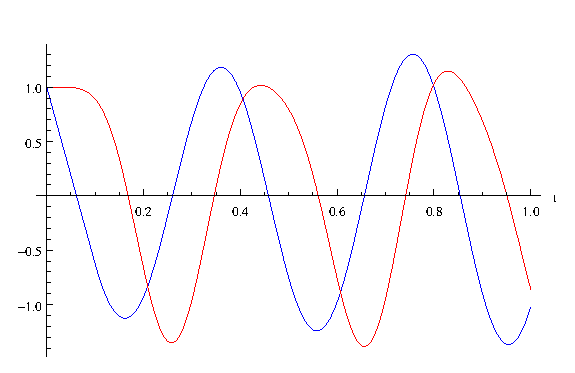
\includegraphics[width=0.65\textwidth]{example_better.eps}
        \end{center}
        \caption{При $\tau=0.1$, $k=4$, $m=5$}
        \end{figure}
    \end{frame}

    \begin{frame}
        \frametitle{Исследование уравнения с запаздыванием}
        \framesubtitle{Сравнение с различными приближениями}

        \begin{figure}[h]
        \begin{center}
            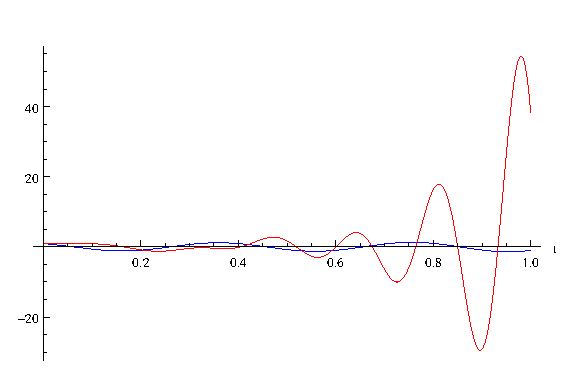
\includegraphics[width=0.65\textwidth]{example_boom.eps}
        \end{center}
        \caption{При $\tau=0.1$, $k=4$, $m=6$}
        \end{figure}
    \end{frame}

    \begin{frame}
        \frametitle{Исследование уравнения с запаздыванием}
        \framesubtitle{Сравнение с различными приближениями}

        \begin{figure}[h]
        \begin{center}
            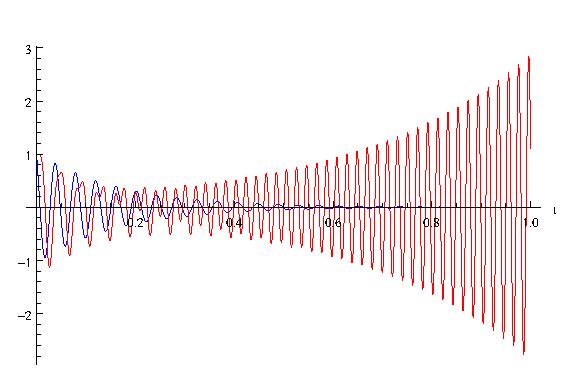
\includegraphics[width=0.65\textwidth]{example.eps}
        \end{center}
        \caption{При $\tau=0.01$, $k=12$, $m=5$}
        \end{figure}
    \end{frame}

    \begin{frame}
        \frametitle{Исследование уравнения с запаздыванием}
        \framesubtitle{Сравнение с различными приближениями}

        \begin{figure}[h]
        \begin{center}
            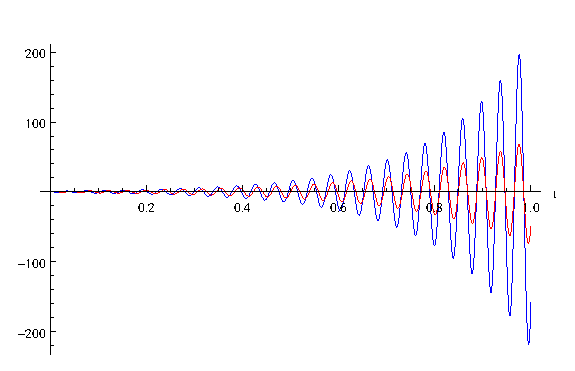
\includegraphics[width=0.65\textwidth]{example_bad.eps}
        \end{center}
        \caption{При $\tau=0.01$, $k=13$, $m=5$}
        \end{figure}
    \end{frame}

    \begin{frame}
        \frametitle{Исследование уравнения с запаздыванием}
        \framesubtitle{Сравнение с различными приближениями}

        \begin{figure}[h]
        \begin{center}
            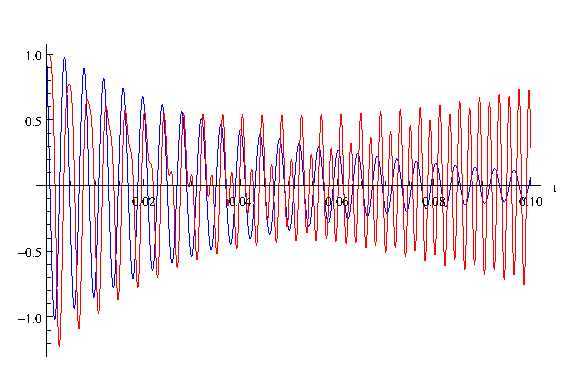
\includegraphics[width=0.65\textwidth]{example_large_good.eps}
        \end{center}
        \caption{При $\tau=0.001$, $k=39$, $m=5$}
        \end{figure}
    \end{frame}

    \begin{frame}
        \frametitle{Исследование уравнения с запаздыванием}
        \framesubtitle{Сравнение с различными приближениями}

        \begin{figure}[h]
        \begin{center}
            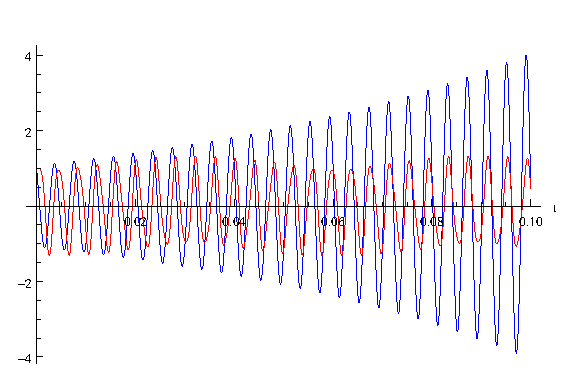
\includegraphics[width=0.65\textwidth]{example_large_bad.eps}
        \end{center}
        \caption{При $\tau=0.001$, $k=40$, $m=5$}
        \end{figure}
    \end{frame}

    \begin{frame}
        \frametitle{Исследование уравнения с запаздыванием}
        \framesubtitle{Сравнение с различными приближениями}

        \begin{figure}[h]
        \begin{center}
            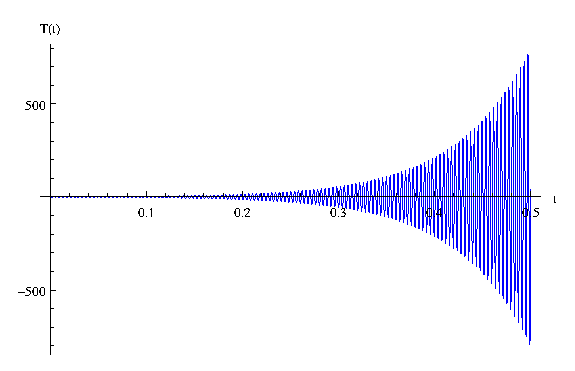
\includegraphics[width=0.45\textwidth]{not_applicable_init.eps}
        \end{center}
        \begin{center}
            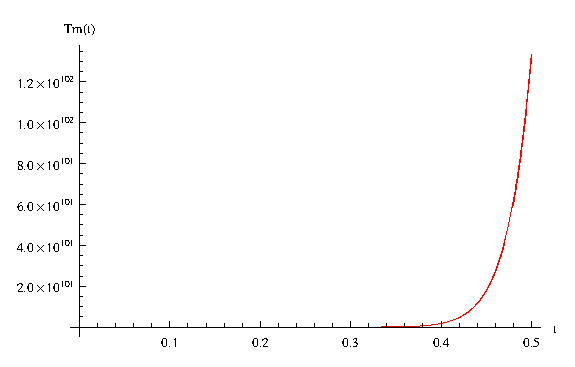
\includegraphics[width=0.45\textwidth]{not_applicable_m.eps}
        \end{center}
        \caption{При $\tau=0.001$, $k=40$, $m=6$}
        \end{figure}

    \end{frame}

    \section{Выводы}

    \begin{enumerate}
    \begin{frame}
        \frametitle{Выводы}

            \item Решения уравнения
                \begin{equation}
                    u_t (x,t) - a^2 u_{xx} (x,t-\tau) + \dfrac{V^2}{4a^2} u (x,t-\tau) = 0
                \end{equation}
                неустойчивы по времени при любой ненулевой начальной функции $T(t)$ при $\tau>0$.

            \item Решения задачи Коши для уравнения с запаздыванием
                \begin{equation}\label{eq:Cauchy}
                \left\{
                    \begin{aligned}
                        T'_k (t) + \underbrace{ \left( \dfrac{V^2}{4a^2} + a^2 k^2 \right)}_{\gamma(k^2)} T_k (t-\tau) = 0, \quad t>0,\\
                        T_k (t) = T_{k}^{0}, \quad -\tau \leq t \leq 0.
                    \end{aligned}
                \right.
                \end{equation}
                устойчивы при $\gamma \tau < 1$ (достаточное условие).

    \end{frame}

    \begin{frame}
        \frametitle{Выводы}

        \item Гипотеза: решения \ref{eq:Cauchy} устойчивы при $\gamma \tau < \dfrac{\pi}{2}$ (необходимое условие).

        \item Приближения для \ref{eq:Cauchy} 
                \begin{equation}
                \left\{
                \begin{aligned}
                    \sum\limits_{n=0}^{m} \dfrac{\tau^n}{n!} T_k^{(n+1)} + \underbrace{ \left( \dfrac{V^2}{4a^2} + a^2 k^2 \right)}_{\gamma(k^2)} T_k = 0, \quad t > 0,\\
                    T_k (0) = T_{k}^{0} \neq 0
                \end{aligned}
                \right.
                \end{equation}
            неустойчивы при $m \geq 6$, устойчивы при $m=1$ при любых $\gamma>0$, $\tau>0$.

    \end{frame}
    \end{enumerate}

    \setbeamertemplate{headline}
    {

    }


    \begin{frame}
        \begin{block}{
            \begin{center}
                \Huge \textbf{СПАСИБО ЗА ВНИМАНИЕ}
            \end{center}
        }
        \end{block}
    \end{frame}

\end{document}